\begin{figure}[H]
    \centering
    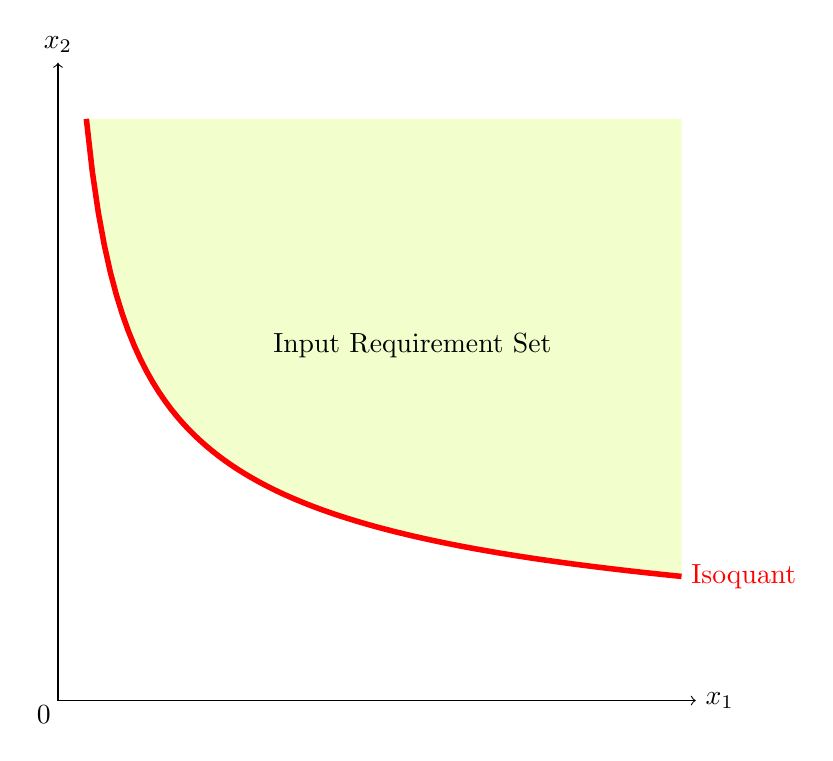
\begin{tikzpicture}[scale=1.8, declare function={f(\x)=1.5^1.5/(\x^0.5);}]
        \path[fill=lime!20] (4.4,1.5^1.5/4.4^0.5) -- (4.4,1.5^1.5/0.2^0.5) -- (0.2,1.5^1.5/0.2^0.5) -- plot[samples=100,variable=\x,domain=0.2:4.4] ({\x},{f(\x)}) -- cycle;
        \draw[->] (0, 0) -- (4.5, 0) node[right] {$x_1$};
        \draw[->] (0, 0) -- (0, 4.5) node[above] {$x_2$};
        \draw[domain=0.2:4.4, samples=100, variable=\x, red, line width=2pt] plot ({\x}, {f(\x)});
        \node at (-0.1,-0.1) {$0$};
        \node[right] at (4.4,1.5^1.5/4.4^0.5) {\color{red} Isoquant};
        \node at (2.5,2.5) {Input Requirement Set};
    \end{tikzpicture}
\end{figure}